\section{Derniers préparatifs}

Date: 11/10/2009

\begin{multicols}{2}

Bonjour à tous !!

C'est reparti pour un tour, je m'envole pour l'Amérique latine cette fois pour aller découvrir la culture Inca et les beaux paysages de la Cordillère des Andes. A l'heure où je vous écrit, il est 21h, dimanche soir et je décolle demain matin à 10 heure pour une boucle de 5 semaines essentiellement au Pérou et en Bolivie, mais rien n'est réellement fixé et il se peut très bien que j'aille faire un petit tour au Chili, en Argentine, au Paraguay ou au Brésil. En fait le choix se fera réellement sur place, en fonction des rencontres, et peut-être aussi des mouvements sociaux (l'Est de la Bolivie est parfois à éviter), je me renseignerai sur place.

Alors sur une carte, ça donne quoi ?

\hspace*{-0.65cm}
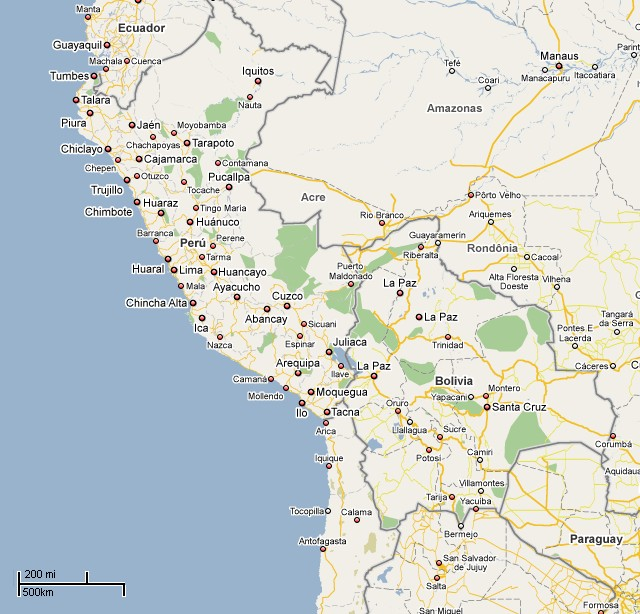
\includegraphics[width=4.8cm]{articles/Derniers-preparatifs/1255286224vDMd.jpg}
Carte du Pérou


J'atterris à Lima mardi matin, à l'aube (ma journée de lundi aura duré 31h), de là je pars vers le sud par la côte, et je pense m'arrêter à Pisco, juste au dessus de Ica. Et la s'arrêtent les plans, vous lirez la suite ici car je ne la connais pas encore...

Allez, si, j'ai deux destinations à aller voir : Le Machu Pichu, situé près de Cuzco et à une altitude telle qu'il faut du temps pour s'y habituer, puis le Salar Uyuni (désert de sel) situé au Sud de la Bolivie, au Sud Ouest de Potosi.

Sur ce je vous dit à bientôt ici même, j'essaierai de mettre un article toutes les semaines environs (sous réserve de cyber cafés disponible).

Etienne

\end{multicols}
